%\documentclass[pdftex,a4paper,12pt]{article}
\documentclass[pdftex,a4paper,10.5pt]{article}

%\usepackage{graphicx}
\usepackage{float}
\usepackage[pdftex]{graphicx}
%\usepackage[latin1]{inputenc}
\usepackage[spanish]{babel}

\pretolerance=2000
\tolerance=3000

\title{\textbf{Algoritmo gen\'etico para la formaci\'on de un equipo}\\
\begin{normalsize}75.70 - Facultad de Ingenier\'ia de la Universidad de Buenos Aires\end{normalsize} }

%\author{ \textbf{Facultad de Ingenier\'ia de la Universidad de Buenos Aires}\\
%\textbf{75.70} \\ \\ 
%Ciancio Alessio, Mauro -% \textit{Padr\'on Nro. 86.357} \\
%\texttt{maurociancio@gmail.com} \\
%Gilioli, Leandro E. -% \textit{Padr\'on Nro. 86.075} \\
%\texttt{legilioli@gmail.com} \\
%L\'opez El\'ias, Lucas -% \textit{Padr\'on Nro. 85.747} \\
%\texttt{lucasdle@gmail.com} \\
%Ucciani, Juan - %\textit{Padr\'on Nro. 86.473} \\
%\texttt{jucciani@gmail.com} \\
%\texttt{njytito@gmail.com} \\
%\texttt{\{maurociancio,legilioli,lucasdle,jucciani,njytito\}@gmail.com} \\[2.5ex]
%}

\author{
	Ciancio Alessio, Mauro \and
	Gilioli, Leandro E. \and
	L\'opez El\'ias, Lucas \and
	Ucciani, Juan Manuel \and
	Yoan, Norberto \\
	\texttt{\{maurociancio,legilioli,lucasdle,jucciani,njytito\}@gmail.com}
	}
	
\date{1er Cuatrimestre de 2010}


\begin{document}
\maketitle

\begin{abstract}
	Desarrollo de una aplicaci\'on que utilice un algoritmo gen\'etico para formar un equipo para el Gran DT bas\'andose en la informaci\'on disponible de los distintos jugadores. Involucra la definici\'on de una funci\'on de aptitud para los jugadores y el uso de bibliotecas que permitan utilizar un algoritmo gen\'etico para obtener uno de los mejores equipos posibles. 
\end{abstract}

\thispagestyle{empty}
%\newpage
%\tableofcontents
%\newpage

\section{Introducci\'on}
El presente trabajo utiliza un algoritmo gen\'etico para la formaci\'on de un equipo de f\'utbol para el GranDT. La aplicaci\'on desarrollada toma los datos hist\'oricos de los jugadores y en base a ellos calcula la funci\'on de aptitud de cada uno. Luego de esto, se corren varias iteraciones del agoritmo gen\'etico aplicando los operadores de selecci\'on, cruza y mutaci\'on para lograr llegar a una poblaci\'on que contenga a los mejores equipos posibles.


\section{Desarrollo}
El documento se encuentra organizado en las siguientes secciones:
\textit{Estado del arte} nos da una idea de las t\'ecnicas actuales utilizadas en aplicaciones similares en el ámbito de algoritmos gen\'eticos. 
\textit{Presentaci\'on del Problema} presenta el dilema a resolver.
\textit{Resoluci\'on} muestra la definici\'on de la soluci\'on planteada para resolver el problema anterior. 
\textit{Resultados} muestra luego de aplicar la soluci\'on a un conjunto de entradas que representa al espectro de entradas posibles, las diferentes salidas de la aplicaci\'on desarrollada.
Finalmente la secci\'on \textit{Conclusiones} muestra el resultado del an\'alisis del funcionamiento de la aplicaci\'on.

\subsection{Estado del arte}
El algoritmo genético es una técnica de búsqueda basada en la teoría de la evolución de Darwin, que ha cobrado tremenda popularidad alrededor del mundo durante los últimos años.
La aplicación más común de los algoritmos genéticos ha sido la solución de problemas de optimización, en donde han mostrado ser muy eficientes y confiables. Los algoritmos genéticos son de probada eficacia en caso de querer calcular funciones no derivables (o de derivación muy compleja) aunque su uso es posible con cualquier función.
Durante los últimos años una gran parte de la investigación en esta área se ha concentrado en el desarrollo de mejoras al desempeño de los algoritmos genéticos. Se han propuesto nuevas técnicas de representación, selección y cruza, con resultados muy alentadores. 
 %estado de la cuestin
%[FUMARse gugle e ieee]

\subsection{Presentaci\'on del Problema}

El problema principal que se intenta resolver es el de determinar los jugadores pertenecientes al equipo ideal para el juego del Gran DT. Uno de los mayores retos para el desarrollo de la aplicaci\'on es la de definir la forma en la que se calcular\'a la funci\'on de aptitud en base a los datos de cada jugador. Adem\'as se deber\'a integrar el c\'odigo con las bibliotecas existentes para la utilizaci\'on de algoritmos gen\'eticos y habr\'a que definir la cantidad de iteraciones o tiempo que el algoritmo realizar\'a para tener una poblaci\'on de individuos que representen un buen resultado (es decir, un buen equipo).

El equipo que se fomrar\'a deber\'a cumplir con las siguientes restricciones:

\begin{itemize}
\item Cantidad de jugadores: todo equipo debe tener 11 jugadores.
\item Costo total: la sumatoria del valor de cada jugador del equipo no puede superar los \$60000000.
\item Clubes: no pueden incluirse en el equipo m\'as de tres jugadores que pertenezcan a un mismo club.
\item Posici\'on de jugadores: debe haber un arquero, cuatro defensores, cuatro mediocampistas y dos delanteros.
\item Jugadores repetidos: cada jugador s\'olo puede ser incluido una sola vez.

\end{itemize}


\subsection{Resoluci\'on}

Para comenzar se recolectaron datos correspondientes a los jugadores y a su desempe\~no durante el campeonato Apertura 2009. Dentro de los datos que se disponene de los jugadores, podemos encontrar \textit{Nombre y Apellido}, \textit{Club}, \textit{Valor del pase}, \textit{Posici\'on} y \textit{puntaje para la fecha n} para las 19 fechas del campeonato. Con estos datos se intentar\'a formar el mejor equipo posible para una determinada fecha, en funci\'on de la informaci\'on disponible en el momento de ejecutar el algortimo.

A continuaci\'on se especifican los par\'ametros utilizados para el algotimo gen\'etico utilizado:

\subsubsection{Cromosoma}

Las posibles soluciones o individos a encontrar tendr\'an una estructura o cromosoma con 11 genes en el que cada gen representa un posible jugador.

\subsubsection{Funci\'on de aptitud}

La funci\'on de aptitud a utilizar para el operador de selecci\'on se dise\~no de forma tal de intentar excluir aquellos individuos que no se ajustan a las restricciones vigentes del problema.

La funci\'on calcular\'a el puntaje o aptitud de una soluci\'on sumando o restando puntos seg\'un se den las siguientes condiciones:

\begin{itemize}
\item Se sumar\'a una cantidad de puntos por cada jugador del equipo igual al promedio de puntos por partido.
\item Si costo del equipo es menor al m\'aximo estipulado, se sumar\'a una cantidad de puntos igual a la diferencia que hay hasta el m\'aximo costo posible.
\item En caso de que no se cumpla alguna de las restricciones del problema, la aptitud de la soluci\'on ser\'a 0.
\end{itemize}

\subsubsection{Selecci\'on}
Se eligi\'o una selecci\'on del tipo elitista para evitar perder las mejores soluciones dado que hay un gran numero de casos en los cuales las soluci\'ones no cumplen con las restricciones del problema. Se intent\'o de esta forma reducir el espacio de b\'usqueda entre las soluciones que las satisfacen.

\subsubsection{Cruza}
Se seleccion\'o la cruza simple, eligiendo al azar uno de los m-1 posibles puntos de cruza del cromosoma para luego intercambiar los segmentos separados por ese punto. Se busc\'o con esta decisi\'on simplificar el proceso de evoluci\'on.

\subsubsection{Mutaci\'on}
Se seleccion\'o una mutaci\'on del tipo simple, es decir, se elige en forma aleatoria un gen, el cual se muta con cierta probabilidad habitualmente muy baja.

\subsubsection{Tama\~no de la poblaci\'on}
Se estableci\'o que la poblaci\'on sobre la cual se va a operar sea de 6 individuos.
 
\subsubsection{N\'umero m\'aximo de iteraciones}
Se limit\'o la cantidad de cilcos de evoluci\'on a 200.


\subsection{Bibliotecas}
La Bibliotecas utilizadas para el desarrollo de la aplicaci\'on son las
siguientes:
\begin{itemize}

\item JGAP : es un componente de algoritmos gen\'eticos y programaci\'on gen\'etica provisto como un framework de Java. Provee mecanismos gen\'eticos basicos que pueden ser usados f\'acilmente para aplicar principios evolutivos a soluciones de un problema.

\end{itemize}
       

\subsection{Resultados} %resultados

Luego del proceso de entrenamiento de la red, se gener\'o una imagen con 27 figuras para probar el funcionamiento de la aplicaci\'on. Estas figuras presentan tama\~nos, orientaciones y geometr\'ias diversas para evaluar el grado de generalizaci\'on alcanzado.

En la figura \ref{salida_ejemlpo} se puede apreciar la salida de la aplicaci\'on en la cual puede verse el correcto funcionamiento de la misma en la gran mayor\'ia de los casos.

 	           \begin{figure}[H]

	                  \begin{center}
	                %	\advance\leftskip-1.5cm
	                  %  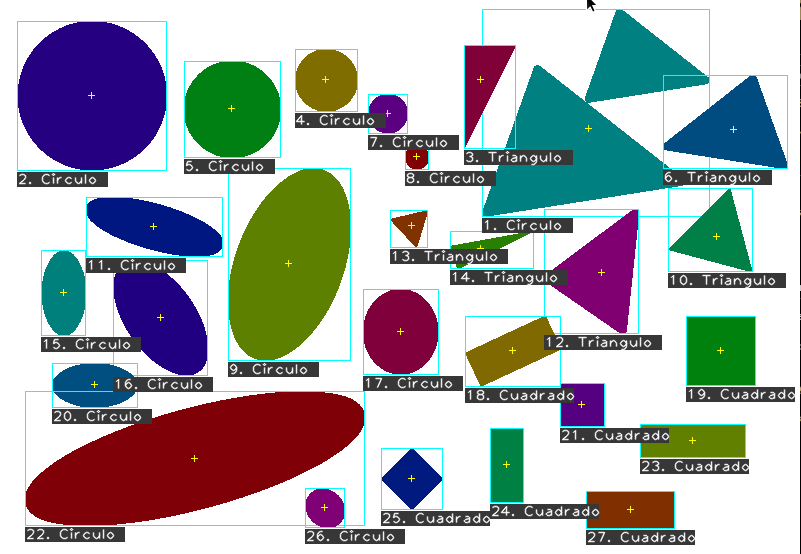
\includegraphics[width=12cm]{salida.png}
	                    \caption{\label{salida_ejemlpo} Salida generada por la aplicaci\'on. }
	                  \end{center}
	            \end{figure}

%\newpage

En la siguiente tabla se pueden apreciar algunos de los datos de entrada y salida de la red neuronal aplicada al caso de prueba presentado.

\begin{table}[ht]
\centering
\begin{tabular}{|l|c|c|c|c|c|c|c|}
  \hline                       
  \textbf{Figura} & \textbf{s1} & \textbf{s2} & \textbf{s3} & \textbf{o1} & \textbf{o2} & \textbf{o3}\\
  \hline
1 & 0.090 & 0.502 & 0.429 & -0.401 & 0.875 & 0.882\\
\hline
3 & 0.030 & 0.525 & 0.299 & 0.000 & 0.964 & -0.020\\
\hline
17 & 0.110 & 0.849 & 0.869 & -0.252 & 0.098 & 0.984\\
\hline
18 & 0.040 & 1.000 & 0.568 & 0.881 & -0.035 & 0.019\\
\hline
19 & 0.040 & 1.000 & 1.000 & 0.911 & 0.010 & 0.011\\

\hline
\end{tabular}	 
\caption{Resultados obtenidos en la corrida de prueba.}
\end{table}

\begin{flushleft}
  $ s_{i}:  $	 \textit{ Entrada de la neurona n\'umero i de la capa de entrada.}\\
  $ o_{i}:  $	 \textit{ Salida de la neurona n\'umero i de la capa de salida. }\\
  $ o_{1}:  $	 \textit{ Corresponde a un cuadrado.}\\
  $ o_{2}:  $	 \textit{ Corresponde a un tri\'angulo.}\\
  $ o_{3}:  $	 \textit{ Corresponde a un c\'irculo.}\\
\end{flushleft}

	        

\newpage
\subsection{Conclusiones} %conclusiones

	En base a los resultados obtenidos, al proceso de desarrollo de la aplicaci\'on y
	entrenamiento de la red podemos elaborar las siguientes conclusiones:
	
	La preparaci\'on de los datos result\'o ser la tarea de mayor complejidad y clave para
	lograr buenos resultados en el reconocimiento. Esto incluye la definici\'on de los atributos
	discriminantes que permitan distinguir a la red entre los distintos tipos de figuras.
	
	Por otro lado, las bibliotecas preexistentes en el mundo del software libre orientadas
	al procesamiento de im\'agenes facilitan la tarea de preparaci\'on y procesamiento 
	de los datos.

	Existen una gran cantidad de herramientas, y el desaf\'io se encuentra en encontrar
	la m\'as adecuada y madura para realizar la tarea deseada.

	La elecci\'on del tipo de red neuronal y la definici\'on de los aspectos antes mencionados
	fue apropiada ya que se obtuvo un alto grado de precisi\'on como puede observarse
	en los resultados expuestos.
	
	El tama\~no de la red no result\'o tan importante como la definici\'on de sus par\'ametros.

\section{Posteriores l\'ineas de Investigaci\'on} %Nuevas lineas de investigacin que se nos fueron ocurriendo

Al presente sistema se le podrían realizar las siguientes mejoras:

\begin{itemize}

\item  Utilizaci\'on de operadores din\'amicos, esto implica que los operadores se modifiquen durante
la ejecuci\'on del proceso, por ejemplo, el operador de mutaci\'on podr\'ia incrementar o reducir
su porcentaje de incidencia en función al resultado que se va obteniendo durante la corrida
del sistema.
\item Modificaci\'on de la funci\'on de aptitud para incluir m\'as restricciones, el sistema podr\'ia tener otros componentes y funcionar en base a otras variables. 
\item Modificar el operador de selecci\'on para orientar la b\'usqueda m\'as r\'apidamente a las soluciones que mejor se adec\'uan a las reglas del problema.
\item Experimentar con otro tipo de cruza para determinar si es posible encontrar una soluci\'on buena en menor tiempo.

\end{itemize}
\newpage

\begin{thebibliography}{9}

\bibitem{martinez}
 García Mart\'inez,
 \emph{Algoritmos Gen\'eticos}.
 Centro de Ingenier\'ia del Software e Ingenier\'ia del Conocimiento
 Instituto Tecnológico Buenos Aires. 

\bibitem{Cantu-Paz}
 Cant\'u-Paz,
 \emph{A Summary of Research on Parallel Genetic Algorithms}.
 IlliGAL Report No. 95007, University of Illinois
 Julio 1995

\bibitem{De Jong}
 De Jong, Spears,
 \emph{A Formal Analysis of the Role of Multi-Point Crossover in Genetic Algorithms}.
Annals of Mathematics and Artificial Intelligence Joumal,
 Vol 5, No. 1, 1992

\bibitem{Goldberg}
 Goldberg,
 \emph{Genetic Algorithms in Search, Optimization, and Machine Learning}.
 Addison-Wesley Publishing Company
 1989
 
\bibitem{Goldberg2}
 Goldberg,
 \emph{Genetic and Evolutionary Algorithms}.
 Age Communications of the
 ACM, Vol. 37, No. 3, 
 Marzo 1994

\bibitem{Goldberg3}
 Goldberg,
 \emph{Genetic Algorithms, Selection Schemes, and the Varying Effects of Noise}.
 IlliGAL Report No. 95009, 
 University of Illinois, 
 1995
 
\bibitem{Spears}
 Spears,
 \emph{Crossover or Mutation}.
 Proceedings of the Foundations of Genetic Algoritluns Workshop Vail, Colorado, pag. 221- 237,
 Julio 1992
 
 \bibitem{jgap}
 JGAP, 
 \emph{Genetic Algorithms and Genetic Programming package}
 Release: 3.4.4,
 Octubre 2009
 

\bibitem{Holland}
 Holland,
 \emph{Schemata}.
  GA-List, GA Vol. 8 No. 26,1994 [MIL/95]
  
\bibitem{Miller}
 Miller,Goldberg, 
 \emph{Genetic Algoriduns, Toumwnent Selection, and the Effects of Noise}.
 IlliGAL Report No. 95006, University of Illinois, 1995
  

  
\end{thebibliography}

%No tiene que tener menos de 7 hojas ni mas de 10
%y en A4 abrochado.
%formato paper.

\end{document}
